%%%%%%%%%%%%%%%%%%%%%%%%%%%%%%%%%%%%%%%%%%%%%%%%%%%%%%%%%%%%%%%%%%%%%%%%%%%
%% This file is part of the book
%%
%% Algorithmic Graph Theory
%% http://code.google.com/p/graph-theory-algorithms-book/
%%
%% Copyright (C) 2009--2011 Minh Van Nguyen <nguyenminh2@gmail.com>
%%
%% See the file COPYING for copying conditions.
%%%%%%%%%%%%%%%%%%%%%%%%%%%%%%%%%%%%%%%%%%%%%%%%%%%%%%%%%%%%%%%%%%%%%%%%%%%

\documentclass{article}

\usepackage{tikz}
\usetikzlibrary{automata}
\usetikzlibrary{external}
\usetikzlibrary{positioning}
\tikzexternalize{DFA-accepting-same-language-as-NFA}

\begin{document}

\begin{figure}
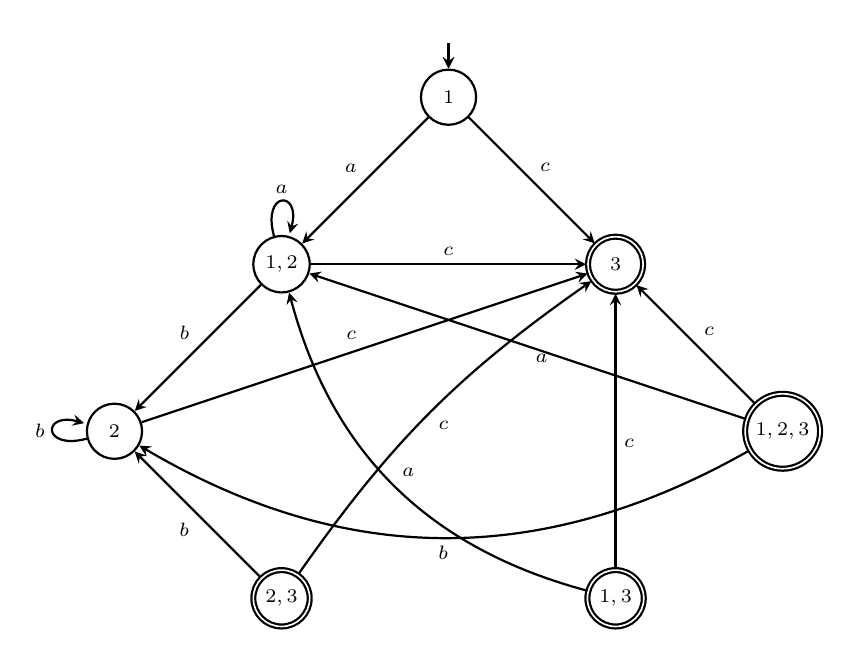
\begin{tikzpicture}
[node distance=3cm,on grid,>=stealth,thick,initial text=,%
  every state/.style={draw,thick}]
\scriptsize
%% nodes or states
\node[state,initial,initial above] (1) {$1$};
\node[state] (12) [below left=of 1] {$1,2$};
\node[state,accepting] (3) [below right=of 1] {$3$};
\node[state,accepting] (123) [below right=of 3] {$1,2,3$};
\node[state] (2) [below left=of 12] {$2$};
\node[state,accepting] (13) [below left=of 123] {$1,3$};
\node[state,accepting] (23) [below right=of 2] {$2,3$};
%% transitions or edges
\path[->,thick]
(1) edge node[above left] {$a$} (12)
(1) edge node[above right] {$c$} (3)
(12) edge[loop above] node {$a$} (12)
(12) edge node[above] {$c$} (3)
(12) edge node[above left] {$b$} (2)
(123) edge node[below right] {$a$} (12)
(123) edge[bend left] node[below] {$b$} (2)
(123) edge node[above right] {$c$} (3)
(2) edge[loop left] node {$b$} (2)
(2) edge node[above left] {$c$} (3)
(13) edge[bend left] node[above right] {$a$} (12)
(13) edge node[below right] {$c$} (3)
(23) edge node[below left] {$b$} (2)
(23) edge[bend left=10] node[below right] {$c$} (3);
\end{tikzpicture}
\end{figure}

\end{document}
